\documentclass[a4paper,10pt]{article}

\usepackage[utf8]{inputenc}
\usepackage{default}
\usepackage{pslatex}
\usepackage{graphicx}
\usepackage{algorithmic}
\usepackage{multicol}
%opening
\title{Comment simuler numériquement la geormphologie de type alpine}
\author{Manceau Thibaut, Gros Alexis, Porteries Tristan}

\begin{document}

\maketitle

\begin{abstract}

\end{abstract}


Avant le TPE nous étions fortement intéressé par la représentation 3D d'un terrain pour des applications telles que les jeux vidéo. Notre intention était donc d'expliquer une grande partie de notre travail déjà fait sur la représentation 3D d'un terrain pré-calculé (environ 6 mois de travail) dans le TPE.

La problématique est 'Comment simuler numériquement la géomorphologie alpine'
'Comment simuler': Le but du TPE est de reproduire des phénomènes naturels.
'numériquement' : Nous n'avons pas les moyens de faire une maquette, donc cette simulation sera  exclusivement réalisé avec de la programmation.
'la géomorphologie' : C'est l'étude de la surface de la terre et de son évolution.
'alpine' : La simulation prendra pour exemple le cas des alpes pour les phénomènes et les types de roches.

Comment on peut le remarquer la problématique ne se prête pas à notre intention initiale ou du moins que pour le résultat final si gain de temps. Partant de cette problématique, nous avons partagés le travail en deux branches principales : l'érosion et la dynamique orogénique (simulation des interactions entre roches.

Dans la partie dédiée a l'érosion on y retrouve des explications sur le phénomène appuyé par des caractéristiques sur les roches et l'application de cet algorithme dans notre simulation.

Quant à elle la branche sur les plaques tectoniques est composée d'une bref description des deux principaux phénomènes : la subduction et l'obduction, ainsi que les différents types de plaque tectonique : continentale et lithosphérique.

Enfin c'est de branches se rejoignent dans la programmation du système de simulation.

Les Cellules

Premièrement nous avons à définir le plus petit élément de cette simulation, dans ce rôle on y trouvera ce qu'on appellera les cellules. Une cellule est un morceau de terrain sphérique ou cubique  d'environs 10 mètres ce qui nous fait un volume de 1000 mètres cube. Ces cellules ont pour caractéristique immuable leur type de roche et comme caractéristiques mutable la plaque tectonique auquel elles appartiennent, leur position et leur force.

Toutes cellules sont disposées sur une grille pour former un grand bloque indépendant des plaques tectoniques. La disposition des cellules à était sujet à controverses, celles ci doivent former une grille carrée ou un grille du type 'nid d'abeilles'? Finalement nous avons choisi la forme en 'nid d'abeilles' car elle permet une équidistance entre les cellules.

En théorie deux cellules dont la distance est inférieur aux deux rayons et qui n'appartiennent pas a la même plaque tectonique, sont considérées en collision. Lorsqu'une cellule est en collision elle reçoit  une force et la propage aux cellules adjacentes, ces cellules adjacentes vont elles même transmettre leur force aux nouvelles cellules adjacentes formant ainsi une onde se propageant a toutes les cellules du même bloc.
Nous nommerons le front les cellules à la périphérie de l'onde. Lors de la propagation de la force dut à une collision.




Ci dessus deux images représentant le front de cellules. La cellule en collision est dessinée en noir en haut a gauche, en violet les cellules inactives, en jaune les cellules faisant parties du front et en bleu les liens entre les cellules.

Interactions entre cellules

	Propagation de la force entre cellules

Pour commencer les cellules doivent connaître toutes les cellules adjacentes pour pouvoir interagir avec elles. Pour cela nous avons utilisé un arbre kd pour optimiser la recherche des cellules, en effet l'arbre kd permet une recherche des points inclut dans une sphère bien plus rapide qu'une simple recherche linéaire.

Pour éviter des interférences entre  les différentes propagations de forces des cellules en collision, nous utilisons des calques uniques contenant un compteur et un vecteur pas cellules, chacun de ces calques sont liés à une cellules en collision.



Ci dessus la représentation de la force lors de la propagation par des trait rouges. Au commencement de la simulation la force de ces cellules est d'environ deux tiers, et à plus de la moitié de la simulation elle est d'environ un quart de la force d'origine.

\begin{center}
  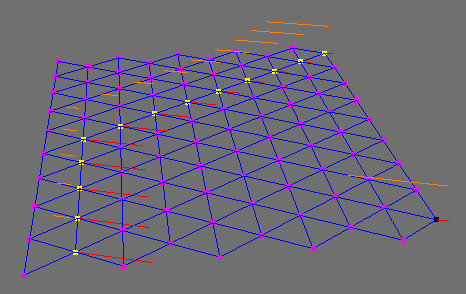
\includegraphics[width=8cm]{screen_calque1.png}
\end{center}

Ci dessus la visualisation des différents calques de force, en rouge la force appliqué par la cellules en collision en haut à gauche et en orange la force pour la cellules en bas à droite.


	Propagation de la force en fonction de l'angle entre cellules

Lorsqu'une cellule propage sa force à ses adjacentes elle doit la partagé pour que le somme de toutes ces forces soit égale à celle d'origine. On doit en aucun cas dans n'importe quelle algorithme avoir plus de forces en sortie qu'en entrée, ce serait totalement illogique car ça signifierait que de la force à était créée. Pour revenir à notre cellule, le partage ne doit pas être équitable car les cellules adjacentes disposées latéralement ne recevront presque aucun force autre que la friction mais au contraire les cellules alignées avec la direction de la force recevront presque la totalité de la force.




$\sum_{i=1}^{n}$





TODO : 
- interaction entre cellules
- collision
- compression
- limite matérielle




\end{document}
